\input{./papers/template.tex}
\usepackage{fitch}
\usepackage{bbm}
\usepackage{stmaryrd}
\usepackage{hyperref}
\usepackage{mathrsfs}
\usepackage{mathtools}
\usepackage{rsfso}
\usepackage{graphicx}
\usepackage[
  backend=biber,
  style=alphabetic,
  sorting=ynt
]{biblatex}
\addbibresource{./refs.bib}
\usepackage{tikz}
\usepackage{tikz-inet}

\author{Alexandra Aiello}
\date{December 19, 2025}
\title{The Dependent Arithmetic Machine}

\begin{document}

\maketitle
\tableofcontents

\section{Abstract}

I present a the Dependent Arithmetic Machine: an implementation of intensional Marin-Löf type theory based on the \(SK\) combinator calculus with a direct correspondence to zero-knowledge algebraic intermediate representations (\textit{ZK-AIR}). I present an arithmetization encoding type-checking in the calculus based on an interpretation of the syntactic category corresponding to the typed calculus as graph constraints in a ZK-AIR. I also outline a \textbf{Lean 4} implementation of the ZK-AIR and demonstrate some interesting properties of it.

\section{Dependent \(SK\) Combinators}

\subsection{Our Type Equations}

\begin{itemize}
  \item \(c(\mathbbm{1}) = 1\)
  \item \(c(I) = 1\)
  \item \(c(K) = 2\)
  \item \(c(S) = 3\)
  \item \(c(MI) = 4\)
  \item \(c(MK) = 5\)
  \item \(c(MS) = 6\)
  \item \(c(Ty_{n}) = n + 6\)
  \item \(MN = c(m) \cdot c(N)\)
\end{itemize}

Edges:

\begin{itemize}
  \item \((1, n + 6)\)
  \item \((1, 4)\)
\end{itemize}

Thoughts:

\begin{itemize}
  \item Need some notion of an atomic expression. Rows are atomics, edges are applications?
  \item Rows = arguments. We need to check all of them. We're not interested in \(\beta\)-reduction
  \item First row = spine
  \item Each atomic element has an ``obvious'' type - we can infer this from the rules
  \item Each argument only has one edge. It's an argument for exactly one node, so we need vertices per row
\end{itemize}

%Example trace:
%
%\begin{tabular}{c c c c}
%  ID & Expr & Edge (app) & Ty\\
%  0 & \(I_{n}\) & N/A & \(MI_{n}\)\\
%  1 & \(MI_{n}\) & 0 & \(\type{n}\)
%\end{tabular}

We can make constraints to make sure each app has exactly the number of arguments we want.
I like our path approach.

If every row has an ``obvious'' type, how do we combine types together?
It's either:
just concatenate them
reduce them

Each element has an obvious type. Apps are what we're concerned with.

Mapping + constraints.
I is just a mapping over the type.
Nondepednent K is just a mapping over the type. We're just exchanging.

Dependent K has extra constraints.

``To follow this path, this path must already exist''. It's a conditional.
There's also beta reduction, we can't foget about that.

What if we mix types and terms?
Assume x is an atomic term. Then, it has a well-known type: \(\langle x, t \rangle\).

Interaction nets idea:

\begin{figure}
  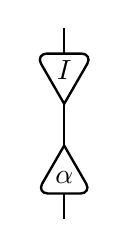
\begin{tikzpicture}[baseline=(current bounding box.center)]
  \matrix[row sep=0.5cm]{
    &\inetcell(I){\(I\)}& \\
    &\inetcell(a){\(\alpha\)}[U]& \\
  };
  \inetwire(I.pal)(a.pal)
  \inetwirefree(I.middle pax)
  \inetwirefree(a.middle pax)
  \end{tikzpicture}
  \hspace{0.75cm}
  \(\mapsto\)
  \hspace{0.75cm}
  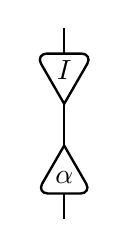
\begin{tikzpicture}[baseline=(current bounding box.center)]
  \matrix[row sep=0.5cm]{
    &\inetcell(I){\(I\)}& \\
    &\inetcell(a){\(\alpha\)}[U]& \\
  };
  \inetwire(I.pal)(a.pal)
  \inetwirefree(I.middle pax)
  \inetwirefree(a.middle pax)
  \end{tikzpicture}
\end{figure}

When we have the requisite number of arguments for a combinator, a constraint applies.

Thought: we don't need to model the types of our base combinators in the ZK-AIR itself.
The AIR is the equivalent of the infer function. The infer function says nothing about our
actual combinator types and values.

These can be rows themselves.
We can create ad-hoc combinators, or inference rules, as long as they are
founded on previous inference rules.

Our core inference rules are encoded in the AIR constraints, but our actual
formulae are lines in the table.

This way we can kind of add more as we see fit.

Equational design is kind of BS, since we can't type-check terms that don't reduce to \(\beta\)-normal forms.
We can use our old meta-combinator hierarchy though. Each one is well-typed even in ``uncurried'' form.

The issue is with typing \(S\). I'm curious to see if we can adapt the de bruijn approach from the CAM paper to LCCC's instead of just CCC's.

With calculus of constructions, we will need to implement contexts and type unification, which is really annoying.

Unflattened meta combintaor approach is really annoying, since dependent \(S\) has a lot of inferene rules.

Munchausen method by Alternkirch \autocite[15]{altenkirch}:

\begin{itemize}
  \item Forward-declarations to postpone value assignments when a type depends on a term
  \item Example: church-encoded dependent product \(\Sigma A B \equiv \lambda (b : Bool), if b then A else B ?\)
    \begin{itemize}
      \item \(?\) is postponed by declaring \(sigma-helper : A\) and accompanying the encoding of the sigma with the rewerite rule \(val : A\ sigma-helper(true) = val\)
      \item We can probably do something similar for combinators, as they showed \autocite[15]{altenkirch}. But we will need to make the theory more ``freestanding'', since their formalism leans on Agda's support for extensionality (UIP?)
    \end{itemize}
\end{itemize}

\printbibliography{}

\end{document}
